%%%%%%%%%%%%%%%%%%%%%%%%%%%%%%%%%%%%%%%%%
% a0poster Landscape Poster
% LaTeX Template
% Version 1.0 (22/06/13)
%
% The a0poster class was created by:
% Gerlinde Kettl and Matthias Weiser (tex@kettl.de)
% 
% This template has been downloaded from:
% http://www.LaTeXTemplates.com
%
% License:
% CC BY-NC-SA 3.0 (http://creativecommons.org/licenses/by-nc-sa/3.0/)
%
%%%%%%%%%%%%%%%%%%%%%%%%%%%%%%%%%%%%%%%%%

%----------------------------------------------------------------------------------------
%	PACKAGES AND OTHER DOCUMENT CONFIGURATIONS
%----------------------------------------------------------------------------------------

\documentclass[a0,landscape]{a0poster}

\usepackage{multicol} % This is so we can have multiple columns of text side-by-side
\columnsep=100pt % This is the amount of white space between the columns in the poster
\columnseprule=3pt % This is the thickness of the black line between the columns in the poster

\usepackage{microtype}
\usepackage{vwcol}
\usepackage{lipsum}
\usepackage[hidelinks]{hyperref}

\usepackage{multirow}


\usepackage[svgnames,table]{xcolor} % Specify colors by their 'svgnames', for a full list of all colors available see here: http://www.latextemplates.com/svgnames-colors

% \usepackage{vwcol}

%\usepackage{times} % Use the times font
\usepackage{palatino} % Uncomment to use the Palatino font

\usepackage{graphicx} % Required for including images
\graphicspath{{figures/}} % Location of the graphics files
\usepackage{booktabs} % Top and bottom rules for table
\usepackage[font=small,labelfont=bf]{caption} % Required for specifying captions to tables and figures
\usepackage{amsfonts, amsmath, amsthm, amssymb} % For math fonts, symbols and environments
\usepackage{wrapfig} % Allows wrapping text around tables and figures
\usepackage{tikz}
\newcommand{\early}{\textsc{Early}~}
\newcommand{\jump}{\textsc{Jump}~}

\newcommand{\eat}[1]{}
% \newcommand{\secmoveup}{\vspace{-1.5cm}}
\newcommand{\secmoveup}{\vspace{-1cm}}
\newcommand{\bibitemmoveup}{\vspace{-.5cm}}
\newcommand{\textmoveup}{\vspace{-.5cm}}
\newcommand{\captionmoveup}{\vspace{-.5cm}}
\newcommand{\itemup}{\vspace{-.5cm}}


\newcommand{\x}{{\mathbf x}}
\newcommand{\bu}{{\mathbf u}}
\newcommand{\vt}{{\mathbf t}}
\newcommand{\cL}{{\cal L}}
\newcommand{\tb}{{\bar t}}
\newcommand{\Tb}{{\bar T}}

\setlength{\columnseprule}{0pt}

\begin{document}

%----------------------------------------------------------------------------------------
%	POSTER HEADER 
%----------------------------------------------------------------------------------------

% The header is divided into three boxes:
% The first is 55% wide and houses the title, subtitle, names and university/organization
% The second is 25% wide and houses contact information
% The third is 19% wide and houses a logo for your university/organization or a photo of you
% The widths of these boxes can be easily edited to accommodate your content as you see fit

\begin{minipage}[m]{0.72\linewidth}
\veryHuge 
%\HUGE 
\color{NavyBlue} \textbf{Probabilistic Knowledge Graph Construction:}  % Title

\Huge\textit{Compositional and Incremental Approaches} % Subtitle

\color{Black}
\vspace{0.5cm}
\huge \textbf{\it Dongwoo Kim, Lexing Xie \& Cheng Soon Ong}, % Author(s)
\huge Australian National University, Data61\\ % University/organization
\end{minipage}
%
\begin{minipage}[m]{0.05\linewidth}

\end{minipage}
%
\begin{minipage}[m]{0.23\linewidth}
\begin{flushright}

\includegraphics[height=5cm]{./logo/anu-logo.jpg}\hspace{.8cm}
\includegraphics[height=5cm]{./logo/DATA61_CSIRO_OnWhite_RGB.jpg}% Logo or a photo of you, adjust its dimensions here
\end{flushright}
\end{minipage}

\vspace{.5cm} % A bit of extra whitespace between the header and poster content

%----------------------------------------------------------------------------------------

\begin{multicols}{3} % This is how many columns your poster will be broken into, a poster with many figures may benefit from less columns whereas a text-heavy poster benefits from more

%----------------------------------------------------------------------------------------
%	ABSTRACT
%----------------------------------------------------------------------------------------

% \color{Navy} % Navy color for the abstract

% \begin{abstract}
%\vspace{.5cm}
% Sed fringilla tempus hendrerit. Vestibulum ante ipsum primis in faucibus orci luctus et ultrices posuere cubilia Curae; Etiam ut elit sit amet metus lobortis consequat sit amet in libero. Lorem ipsum dolor sit amet, consectetur adipiscing elit. Phasellus vel sem magna. Nunc at convallis urna. isus ante. Pellentesque condimentum dui. Etiam sagittis purus non tellus tempor volutpat. Donec et dui non massa tristique adipiscing. Quisque vestibulum eros eu. Phasellus imperdiet, tortor vitae congue bibendum, felis enim sagittis lorem, et volutpat ante orci sagittis mi. Morbi rutrum laoreet semper. Morbi accumsan enim nec tortor consectetur non commodo nisi sollicitudin. Proin sollicitudin. Pellentesque eget orci eros. Fusce ultricies, tellus et pellentesque fringilla, ante massa luctus libero, quis tristique purus urna nec nibh.
%
% \end{abstract}

%----------------------------------------------------------------------------------------
%	INTRODUCTION
%----------------------------------------------------------------------------------------

%\color{SaddleBrown} % SaddleBrown color for the introduction

% \section*{Highlights}
% We proposed methods to predict YouTube viewcount with the feed of Twitter in the cases which can hardly be done with classical methods,
% \begin{itemize}
% \item \early : viewcount shortly after the upload of a new video
% \item \jump : a sudden increase in viewcount
% \end{itemize}

\small

\color{DarkSlateGray}

\noindent\textbf{\Large Motivation}

\vspace{.2cm}

\begin{tabular}{p{\linewidth}}
\cellcolor{DarkSlateGray}
\color{white}
\begin{itemize}
\itemup
\item How to measure \textbf{uncertainty} of unknown facts from observations.
\item How to incorporate \textbf{path structure} into a knowledge graph factorisation to improve  unknown facts prediction.
\item How to balance exploration and exploitation in \textbf{incremental knowledge population}.
\itemup
\end{itemize}
\end{tabular}

\vspace{.5cm}

\noindent\textbf{\Large Contributions}

\vspace{.2cm}

\begin{tabular}{p{\linewidth}}
\cellcolor{DarkSlateGray}
\color{white}
\begin{itemize}
\itemup
\item Propose a \textbf{probabilistic formulation} of bilinear tensor factorisation that allows us to predict the uncertainty of unknown facts.
\item Incorporate the graph \textbf{path structure} of knowledge graph into factorisation by modelling a composition of relations.
\item Develop an incremental population method that searches the factorised space, trading of exploration and exploitation using \textbf{Thompson sampling}.
\itemup
\end{itemize}
\end{tabular}


%----------------------------------------------------------------------------------------
%	OBJECTIVES
%----------------------------------------------------------------------------------------

%\color{DarkSlateGray} % DarkSlateGray color for the rest of the content
\color{Black}


\section{Compositional Relational Model}
A triple, e.g. \{Obama, president of, US\}, is a basic unit of a knowledge graph. A collection of knowledge triples can be represented as a 3d tensor where each dimension represent entity, relation, and entity, respectively. The goal of statistical relational models is to factorise this tensor to obtain low dimensional representations of entities and relations.

\vspace{.5cm}
\noindent\textbf{Probabilistic bilinear factorisation model}

\begin{tabular}{l l}
\begin{minipage}{.60\linewidth}
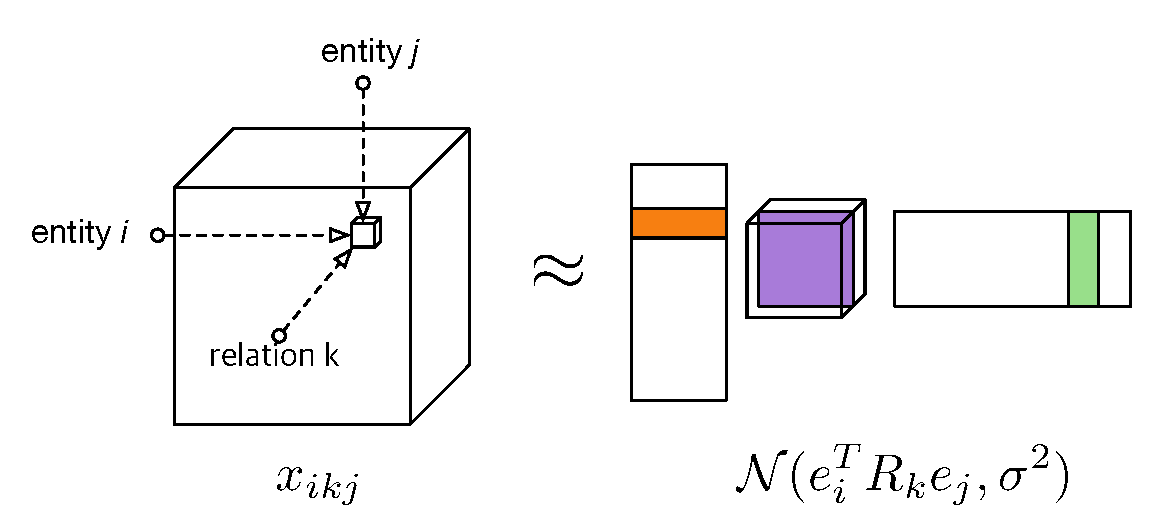
\includegraphics[width=\linewidth]{./figures/rescal.pdf}
\end{minipage}\hspace{1cm}
& 
\begin{minipage}{.34\linewidth}
\captionof{figure}{Illustration of widely used bilinear factorisation model, \textsc{rescal}, where entities are embedded into $D$-dimensional latent space.}
\vspace{-1.5cm}
\begin{equation}
e_i, e_j\in\mathbb{R}^{D}, \quad R_k \in \mathbb{R}^{D\times D} \notag
\end{equation}
\end{minipage}
\end{tabular}

\vspace{.5cm}

We reformulate popular \textsc{rescal} model in a probabilistic way by placing isotropic normal prior over entity vectors and relation matrices. For observations, we use the normal distribution as in figure 1 \textsc{(pnormal)} and logistic function \textsc{(plogit)}.

\vspace{.5cm}
\noindent\textbf{Compositional triples}

\begin{center}
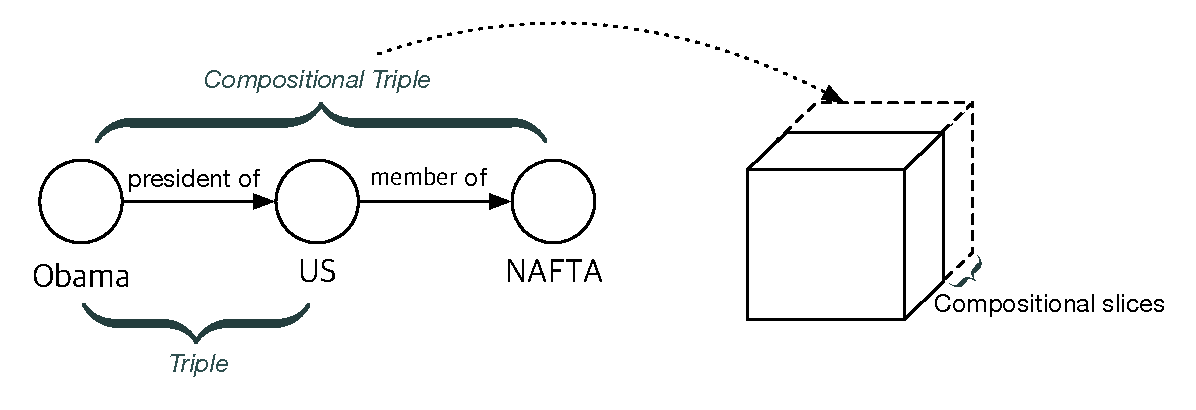
\includegraphics[width=.9\linewidth]{./figures/composition.pdf}
\captionof{figure}{Composition of multiple triples can be interpreted as a compositional triple. We augment the original tensor with these additional triples to incorporate explicit path structure into factorisation.}
\end{center}

Adding compositional slices will increase the number of relation parameters exponentially. Therefore, we propose two different structures to model the compositionality in the latent embedding spaces.

1. Multiplicative compositionality (\textsc{pcomp-mul}):
\begin{align}
x_{icj} \sim \mathcal{N}(e_i^T R_{c_1} R_{c_1} \dots R_{c_n} e_j,\sigma^2)
\end{align}

2. Additive compositionality (\textsc{pcomp-add}):
\begin{align}
x_{icj} \sim \mathcal{N}(e_i^T \frac{1}{c_n} (R_{c_1} + R_{c_1} + \dots + R_{c_n}) e_j,\sigma^2),
\end{align}
where $c$ is a compositional relation with composition of relations $\{c_1, c_2, ..., c_n\}$.


\section{Knowledge Completion}

We first evaluate our model to \textbf{predict unknown triples} given observations to measure the performance of proposed models with all non compositional and compositional variants. For this experiments, we divide datasets into training and testing, and then measure ROC-AUC scores on the test set.

\vspace{.5cm}

\noindent\textbf{Datasets}
We use three benchmark datasets for experiments.
\begin{center}
\begin{tabular}{l | r | r | r | r}
Dataset &  \# rel & \# entities & \# triples & sparsity \\ \hline
Kinship & 26 & 104  & 10,790 & 0.038 \\
UMLS & 49 &135  & 6,752 & 0.008 \\
Nation & 56 & 14  & 2,024 & 0.184 \\
\end{tabular}
\captionof{table}{Description of datasets.
Sparsity denotes the ratio of valid triples to invalid triples.}
\end{center}


\vspace{.5cm}

\begin{tabular}{l l}
\begin{minipage}{.55\linewidth}
%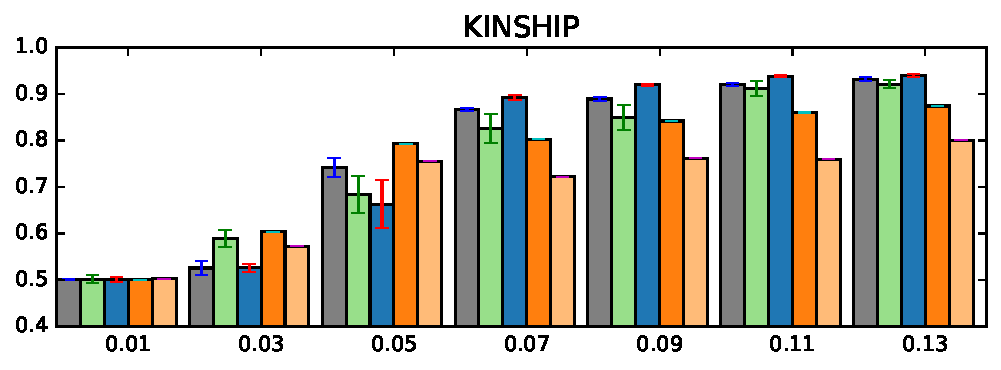
\includegraphics[width=\linewidth]{../cikm2016/images/comp_training_error_kinship_small.pdf}
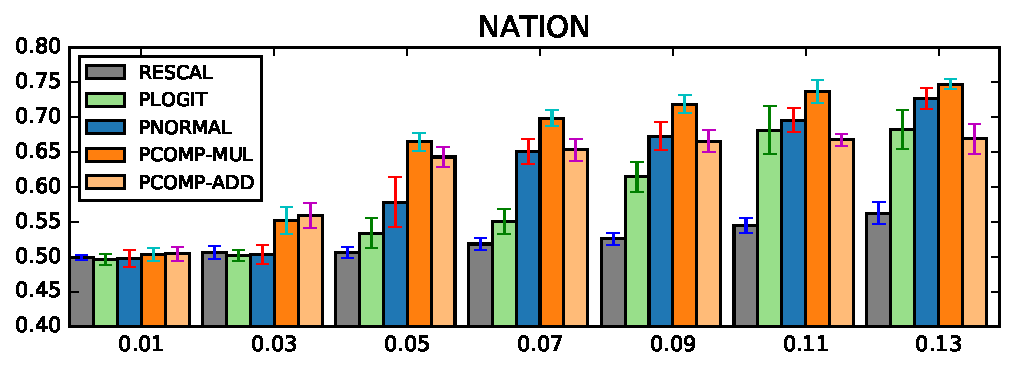
\includegraphics[width=\linewidth]{../cikm2016/images/comp_training_error_nation_small.pdf}
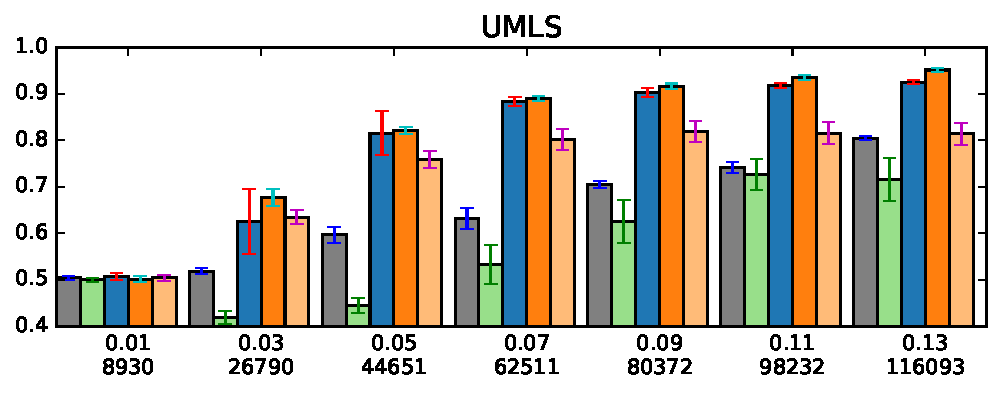
\includegraphics[width=\linewidth]{../cikm2016/images/comp_training_error_umls_small.pdf}
\end{minipage}\hspace{0.5cm}
&
\begin{minipage}{.39\linewidth}
\captionof{figure}{ROC-AUC scores of compositional and non-compositional models. The x-axis denotes the proportion and total number of triples used for training.
\textsc{pnormal} or \textsc{plogit} generally outperform \textsc{rescal}. In general, the multiplicative compositional model \textsc{(pcomp-mul)} outperforms the additive compositional model \textsc{(pcom-add)}, and performs better the other baseline models.}
\end{minipage}
\end{tabular}

\vspace{.5cm}

\noindent\textbf{Compositional path reconstruction}

\vspace{.5cm}

\noindent The goal of the compositional models is to factorise triples along with the graph structure as a whole. To show that the model embeds the graph structure into latent space, we evaluate a path reconstruction task where the model predicts a final entity given source entity and sequence of relations.

\vspace{.5cm}

\begin{tabular}{l l}
\begin{minipage}{.55\linewidth}
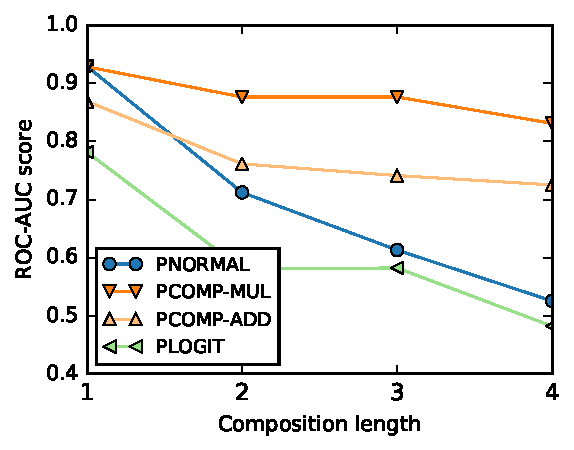
\includegraphics[width=\linewidth]{../cikm2016/images/path_prediction2.pdf}
\end{minipage}\hspace{1cm}
& 
\begin{minipage}{.39\linewidth}
\captionof{figure}{Path prediction result of UMLS. The performances of both compositional models remain consistent whereas those of the non-compositional models drop sharply as the length increases.}
\end{minipage}
\end{tabular}

\vspace{.5cm}

\noindent\textbf{Visualisation of learned entities}

\vspace{.5cm}

\begin{center}
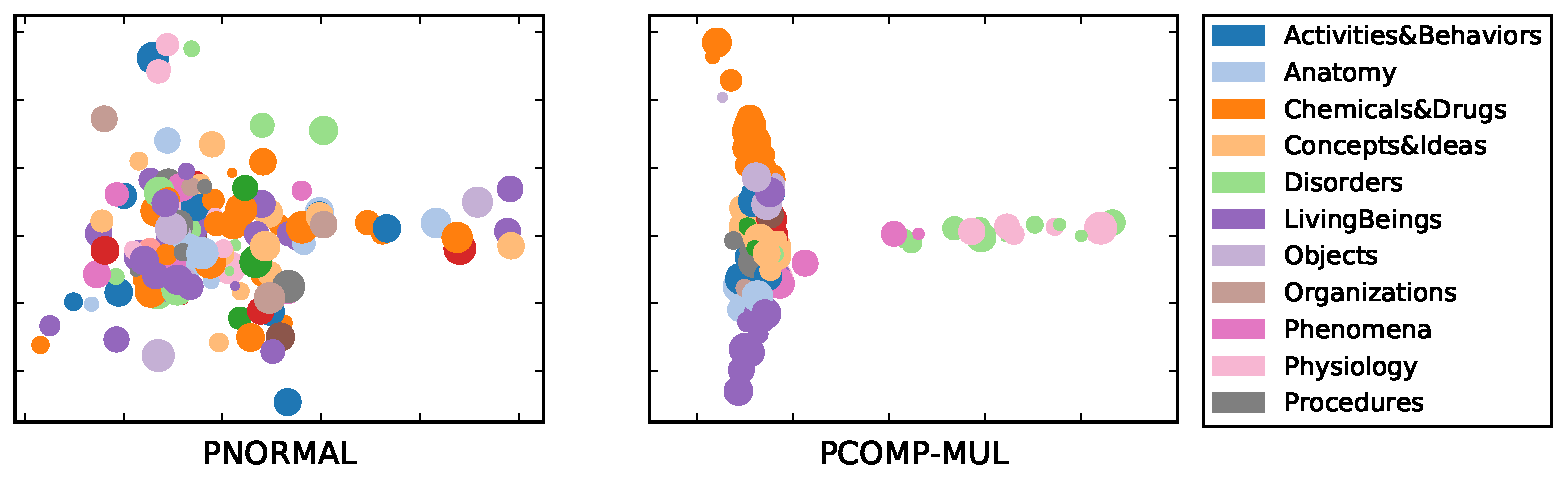
\includegraphics[width=0.9\linewidth]{../cikm2016/images/embedding_umls.pdf}
\captionof{figure}{Embedding learned entities of the UMLS dataset into a two-dimensional space through the spectral clustering. Entities with the same type are represented by the same color.
The entities with the same type are located closer to each other with the multiplicative compositional model (\textsc{pcomp-mul}) than the non-compositional model.
}
\end{center}


\section{Incremental Knowledge Population}

The goal of \textbf{incremental population} is to maximise the number of positive triples based on the interaction between human experts and labels given a limited amount of budget.

A recent attempt at incremental knowledge population (Jiang et al., 2015), has had difficulties simultaneously achieving high recall and faithful reconstruction. We employ \textbf{Thompson sampling}, an approach for solving the multi-armed bandit problem, to find an optimal trade-off between exploration and exploitation during incremental population.

\begin{center}
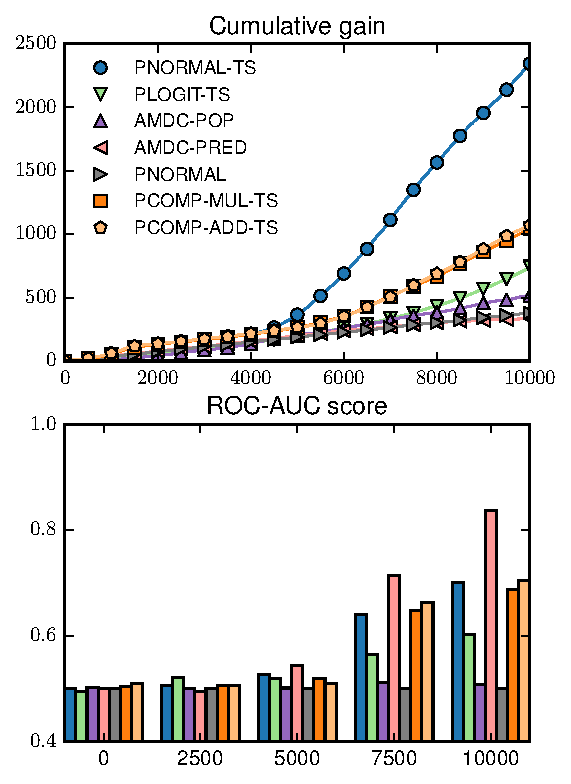
\includegraphics[width=0.32\linewidth]{../cikm2016/images/thompson_kinship_mcmc_vertical_line.pdf}
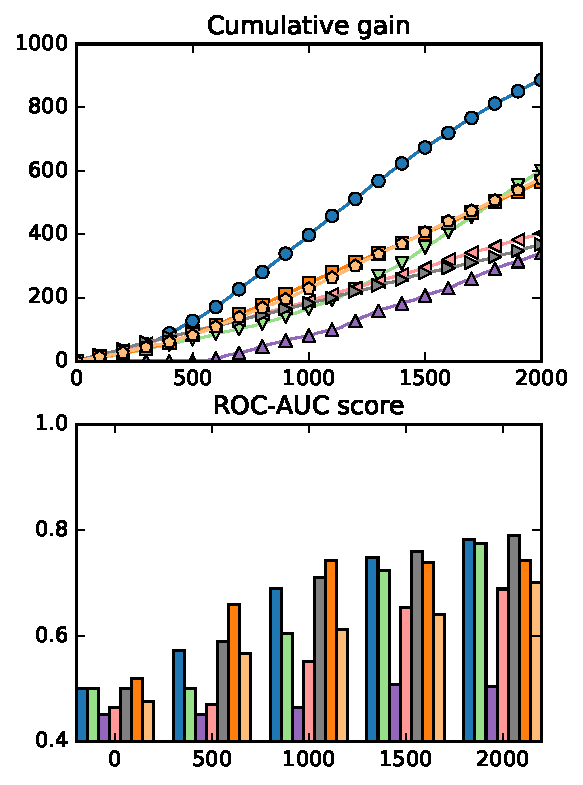
\includegraphics[width=0.32\linewidth]{../cikm2016/images/thompson_nation_mcmc_vertical_line.pdf}
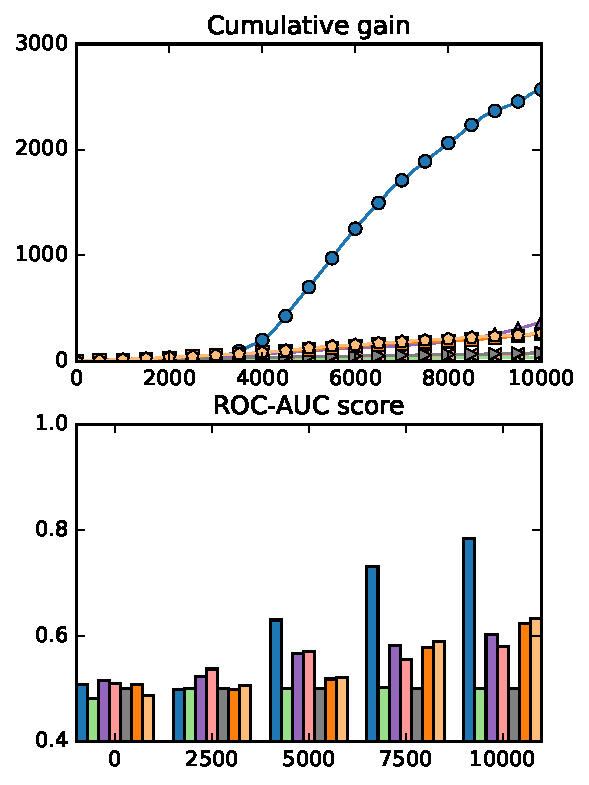
\includegraphics[width=0.32\linewidth]{../cikm2016/images/thompson_umls_mcmc_vertical_line.pdf}
\captionof{figure}{The cumulative gain (upper) and ROC-AUC score (lower) of the Thompson sampling with passive learning and \textsc{amdc} models. X-axis denotes the number of queries issued. Thompson sampling with \textsc{pnormal} model achieves the highest cumulative gain to compare with \textsc{amdc} and passive learning algorithms and shows comparable performance on ROC-AUC scores. The compositional model performs worse than the non-compositional models.}
\end{center}

\secmoveup
\section{Discussion}
Lorem ipsum dolor sit amet, consectetur adipiscing elit. Nullam non lectus vel diam congue tincidunt malesuada sit amet augue. Proin non venenatis odio. Quisque porttitor dolor ut cursus gravida. Integer a iaculis massa. Donec semper leo sed metus tempor varius. Donec mollis risus pharetra ligula lacinia, vitae suscipit arcu vulputate. Pellentesque vel odio tristique, luctus nisl in, elementum tortor. Praesent vitae neque id sapien porta interdum.

%Aliquam dignissim nisl neque, vel interdum leo blandit et. Vivamus sed tincidunt arcu. Vivamus sed tristique ipsum, eu blandit magna. Praesent nec imperdiet nibh. Nullam dignissim dui ac arcu sollicitudin congue. Suspendisse facilisis nulla convallis pellentesque tempus. Vestibulum ante ipsum primis in faucibus orci luctus et ultrices posuere cubilia Curae; Curabitur iaculis gravida enim, id accumsan augue lacinia a. Donec at augue sagittis, imperdiet purus ut, eleifend tortor. Phasellus efficitur ipsum magna, ac ultrices erat pellentesque a. Maecenas sed dui pretium, euismod enim vitae, aliquam dui. Vestibulum vel bibendum arcu. Praesent ac enim bibendum, pharetra ante nec, iaculis lorem. Nunc tempus risus eget enim volutpat, et pulvinar eros porttitor. Morbi dui nisi, vestibulum sed nisl vel, rhoncus tincidunt quam.

%Sed tristique lacus iaculis faucibus lobortis. Aenean mollis sem cursus, blandit lectus at, imperdiet diam. Mauris iaculis, felis id laoreet eleifend, dolor nibh porta nisi, sagittis venenatis ipsum massa eu tellus. Nulla ullamcorper, mi in viverra malesuada, magna urna vulputate elit, ac aliquam massa justo ut urna. Fusce eget mauris commodo, volutpat erat ac, dignissim sapien. Sed lacus felis, pellentesque mollis mattis in, luctus id orci. Morbi in est vehicula, auctor nunc eu, aliquet augue.

%Quisque eu tortor in ligula bibendum rhoncus. Pellentesque dui augue, vulputate at vulputate nec, tempus non diam. Sed et cursus erat. Aliquam erat volutpat. Aliquam quis auctor ipsum. Sed sed nunc sit amet justo laoreet accumsan. Praesent eu ultrices enim, ac tempus sem. Vivamus finibus enim nec nunc fermentum, vel interdum dui maximus. Maecenas faucibus vulputate nisi, vel pharetra turpis auctor non. Etiam ut augue eu augue gravida eleifend.
%
%Cras efficitur lectus neque, dapibus vehicula augue pulvinar non. Aenean hendrerit tellus a nisl accumsan pulvinar. Pellentesque nisl dolor, eleifend et urna a, suscipit tempor orci. Praesent metus velit, tincidunt ac odio ut, elementum convallis nunc. Suspendisse potenti. Lorem ipsum dolor sit amet, consectetur adipiscing elit. Suspendisse ac arcu nunc.



% \begin{thebibliography}{5}
% %\bibitem{everyoneisinfluencer}
% %E.~Bakshy, J.~M. Hofman, W.~A. Mason, and D.~J. Watts.
% %\newblock Everyone's an influencer: quantifying influence on twitter.
% %\newblock WSDM '11, pages 65--74, 2011.
%
% \bibitemmoveup
% \bibitem{crane2008robust}
% R.~Crane and D.~Sornette.
% \newblock Robust dynamic classes revealed by measuring the response function of a social system.
% \newblock Proc. Natl. Aca. Sci., vol 105 no 41, pages 15649-53, 2008
%
% \bibitemmoveup
% \bibitem{kwak2010twitter}
% H.~Kwak, C.~Lee, H.~Park, and S.~Moon.
% \newblock What is twitter, a social network or a news media?
% \newblock In {\em WWW}, pages 591--600. 2010.
%
% \bibitemmoveup\bibitem{pinto2013}
% H.~Pinto, J.~M. Almeida, and M.~A. Gon\c{c}alves.
% \newblock Using early view patterns to predict the popularity of youtube
%   videos.
% \newblock WSDM '13.
%
% \bibitemmoveup\bibitem{acmcompaper}
% G.~Szabo and B.~A. Huberman.
% \newblock Predicting the popularity of online content.
% \newblock {\em Commun. ACM}, 53(8):80--88, Aug. 2010.
%
% \bibitemmoveup\bibitem{yang2011patterns}
% J.~Yang and J.~Leskovec.
% \newblock Patterns of temporal variation in online media.
% \newblock WSDM 2011. %pages 177--186, 
% \end{thebibliography}

\end{multicols}
\end{document}
%%% Local Variables:
%%% mode: latex
%%% TeX-master: t
%%% End:
